\section{Empirical Application: Additional Results}\label{sec:app_empirical}

\subsection{Classifier construction}\label{sec:app_classifier}

The binary group indicator $G^*_d$ is constructed separately for each district $d$ in three steps, following \cite[][Section 5.2]{fuzzy2018}.

\paragraph{Step 1: Contingency table.} Cross-tabulate individuals in district $d$ by years of schooling and cohort into cell counts $n_{d,k,c}$, where $k \in \{0, 1, \ldots, 18\}$ indexes \texttt{yeduc} and $c \in \{0, 1\}$ indexes the young-cohort indicator.

\paragraph{Step 2: Chi-squared test of independence.} The null is that \texttt{yeduc} and \texttt{young} are independent in district $d$, which means the schooling distribution is the same in the old and young cohorts. The test statistic is
\begin{equation*}
\chi^2_d = \sum_{k,\,c} \frac{(n_{d,k,c} - E_{d,k,c})^2}{E_{d,k,c}}, \qquad E_{d,k,c} = \frac{n_{d,k,\cdot}\,n_{d,\cdot,c}}{n_{d,\cdot,\cdot}},
\end{equation*}
which has approximately a $\chi^2$ distribution with degrees of freedom equal to one less than the number of nonempty \texttt{yeduc} rows. Let $p_d$ denote the p-value. Rejecting $H_0$ flags district $d$ as having a cohort-level shift in the schooling distribution.

\paragraph{Step 3: Sign the rejection.} The test is two-sided, so \citeauthor{fuzzy2018} sign each rejection by the direction of the change in mean schooling between cohorts,
\begin{equation*}
G^*_d = \begin{cases}
+1 & p_d < 0.5 \text{ and } \overline{\text{yeduc}}_{d,\text{young}} > \overline{\text{yeduc}}_{d,\text{old}}, \\
-1 & p_d < 0.5 \text{ and } \overline{\text{yeduc}}_{d,\text{young}} < \overline{\text{yeduc}}_{d,\text{old}}, \\
\phantom{+}0 & p_d \geq 0.5.
\end{cases}
\end{equation*}

\paragraph{Interpretation.} $G^*_d = +1$ marks districts where INPRES plausibly shifted schooling upward, which are the treatment group in this paper. $G^*_d = 0$ marks districts with no detectable cohort shift, the control group. $G^*_d = -1$ marks districts where schooling shifted downward for reasons unrelated to INPRES. This paper drops $G^*_d = -1$ districts because Theorem~\ref{thm:1} is stated for binary $G$. The threshold $p_d < 0.5$ is a classification cutoff, not a conventional significance test. It is chosen to label every district as one of $\{-1, 0, +1\}$ rather than to provide inference on whether a shift occurred.

\subsection{Sample and classifier}\label{sec:app_sample}

I use the 1995 Indonesian Intercensal Survey (SUPAS) microdata from \citet{duflo2001schooling}. The sample pools both sexes with non-missing log hourly wage, born in 1957--1962 (old cohort, $T=0$) or 1968--1972 (young cohort, $T=1$). Years of schooling is top-coded at $18$ (recoding $19 \to 18$ to match the \citeauthor{fuzzy2018} replication). The outcome $Y$ is log hourly wage and the classifier $G^*$ is the chi-squared test on the full $\text{yeduc} \times \text{young}$ contingency table at threshold $p < 0.5$, signed by the change in mean years of schooling. The paper's theorem is stated for binary $G$, so I restrict to $G^* \in \{0, 1\}$ and drop the $G = -1$ districts. Table~\ref{tab:classifier} compares classifier counts to \cite{duflo2001schooling} and \cite{fuzzy2018}.

\begin{table}[H]
    \centering
    \small
    \input{../output/tables/empirical_classifier.tex}
    \caption[District classifier comparison]{District classifier comparison. \cite{duflo2001schooling} uses continuous INPRES intensity as an instrument and has no binary $G^*$. \cite{fuzzy2018} Table~3 reports counts $97/64/123$; ours are $96/67/127$, within $\pm 4$ districts due to boundary drift between R's \texttt{chisq.test} and Stata's \texttt{tab2, chi2}. \citeauthor{fuzzy2018} pool $G^* \in \{-1, 0, +1\}$ via a mirror Wald formula and report on the full 284-district sample. This paper's theorem handles binary $G$, so I restrict to $G^* \in \{0, 1\}$, which gives $N = 22{,}414$ observations in $201$ districts.}\label{tab:classifier}
\end{table}

\subsection{Covariate dictionary and excluded variables}\label{sec:6c}

The dictionary contains $p = 45$ individual-level regressors: sex, birth year interacted with cohort, Java residence at birth, urban residence at birth, and their pairwise interactions. These vary within both $G = 0$ and $G = 1$ districts and keep $\hat e(X)$ strictly interior on the full sample (Figure~\ref{fig:propensity_app}). Estimation uses observation-level cross-fitting with $L = 5$ folds and cluster-robust standard errors at the district of birth following Remark~\ref{rem:cluster}.

District-level statistics that summarize the cohort-by-education distribution (mean education of older cohorts, 1971 enrollment rate, 1971 children population) are excluded because they pin $\Pr(G = 1 \mid X) \in \{0, 1\}$ by construction, driving $\hat e(X)$ to the boundary and emptying holdout cells after trimming. Pre-INPRES district variables correlated with the INPRES allocation rule (program intensity, 1971 population density, water and sanitation spending) are also excluded because conditioning on them absorbs the first-stage variation that identifies the LATE.

\subsection{Descriptive statistics and diagnostics}\label{sec:app_descriptives}

\begin{table}[H]
    \centering
    \input{../output/tables/empirical_balance.tex}
    \caption[Descriptive statistics by group-time cell]{Descriptive statistics by group-time cell. $G=1$ districts experienced a significant cohort shift in the education distribution with rising schooling; $G=0$ districts did not. $T=0$ is the old cohort (1957--1962, unexposed to INPRES), $T=1$ the young cohort (1968--1972, exposed). $Y$ is log hourly wage; $D = \mathbf{1}\{\text{years of schooling} \geq 6\}$. District-level covariates are from 1971 census data. Standard deviations in parentheses.}\label{tab:balance}
\end{table}

\begin{figure}[H]
    \centering
    \begin{subfigure}[b]{0.48\linewidth}
        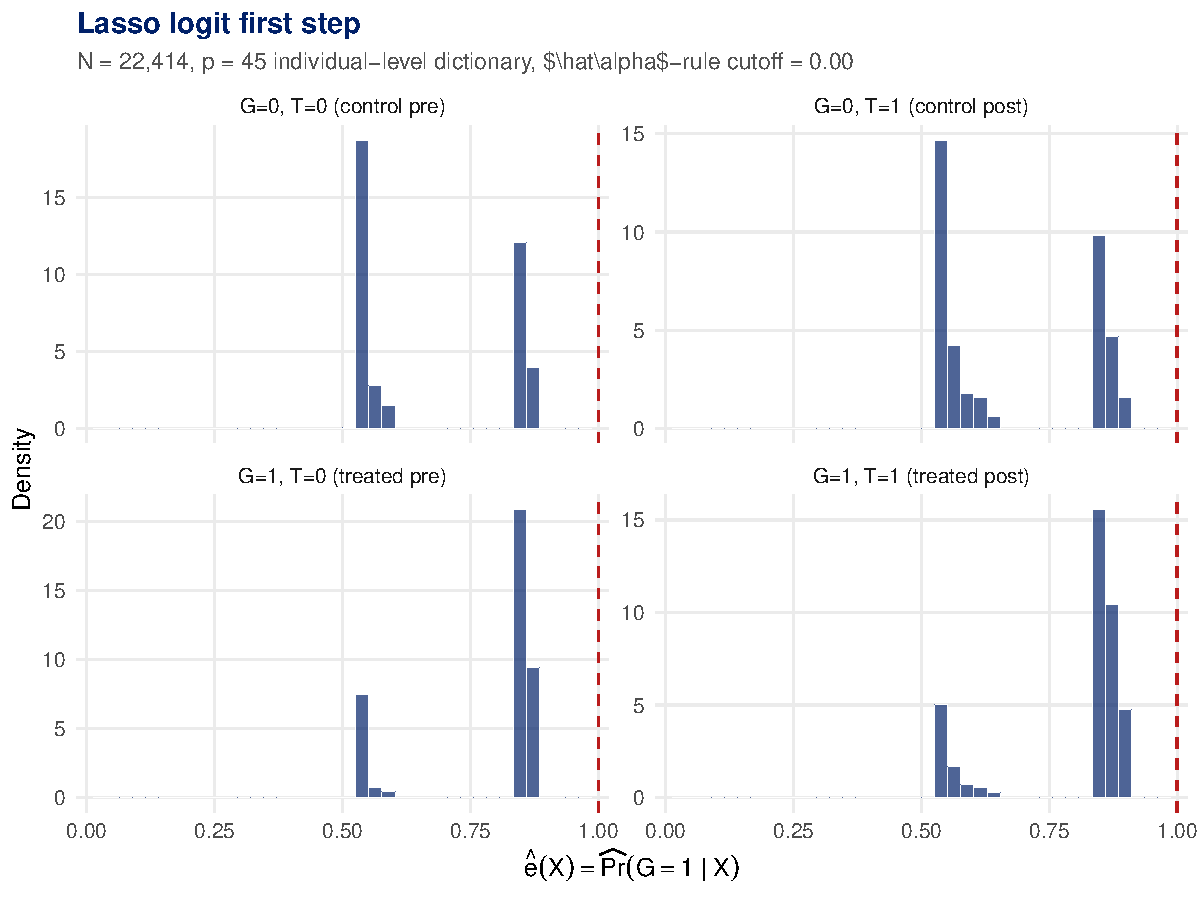
\includegraphics[width=\linewidth]{../output/figures/empirical_propensity_lasso.pdf}
        \caption{Logit-Lasso first step.}\label{fig:propensity_lasso}
    \end{subfigure}
    \hfill
    \begin{subfigure}[b]{0.48\linewidth}
        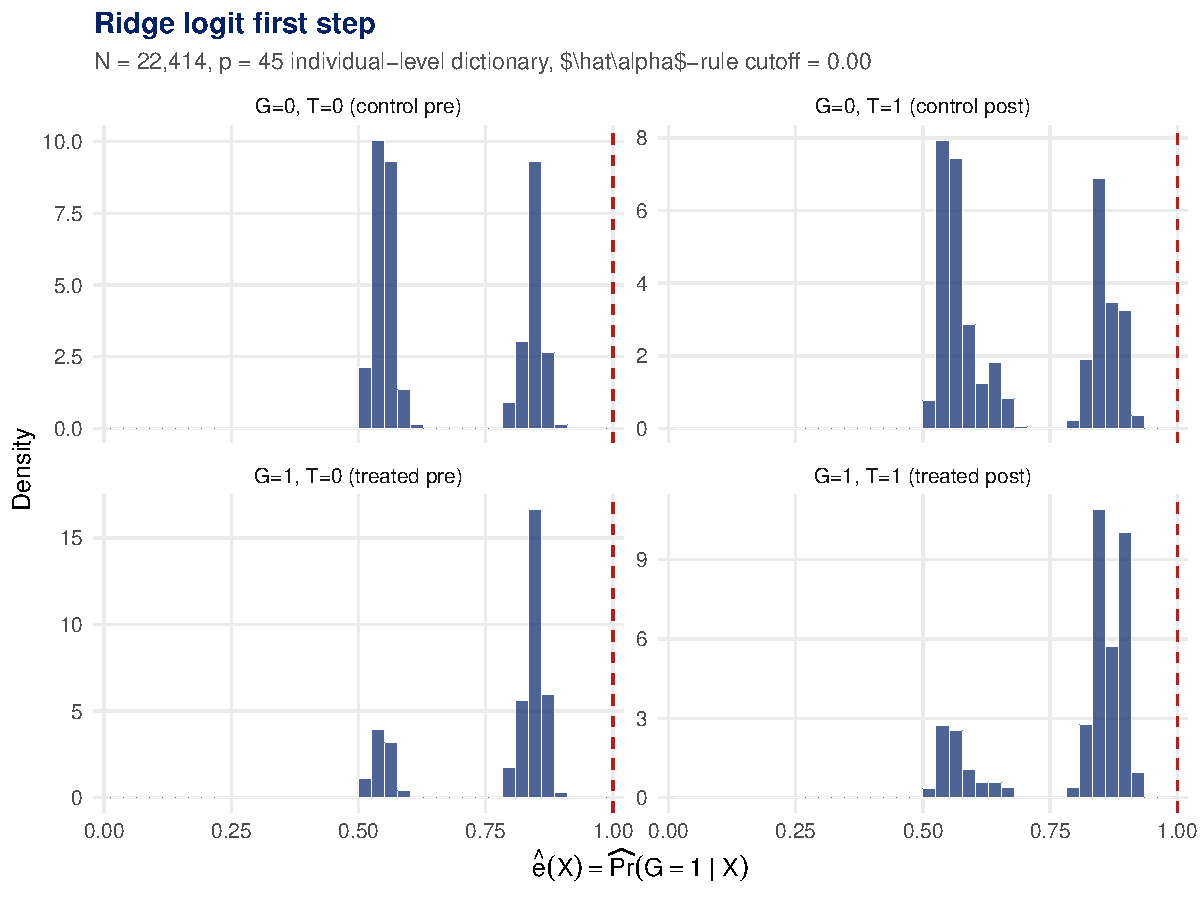
\includegraphics[width=\linewidth]{../output/figures/empirical_propensity_ridge.pdf}
        \caption{Logit-Ridge first step.}\label{fig:propensity_ridge}
    \end{subfigure}
    \caption[Propensity score distribution by $(G,T)$ cell]{Distribution of $\hat e(X) = \hat{\Pr}(G=1 \mid X)$ by $(G,T)$ cell on the $p=45$ individual-level dictionary ($N = 22{,}414$). Both Lasso and Ridge produce interior propensities with no mass at the boundary. Lasso range $[0.53, 0.91]$ with mean $0.77$ and SD $0.14$; Ridge range $[0.51, 0.91]$ with mean $0.77$ and SD $0.14$. The share above $0.9$ is $1\%$ under Lasso and $6\%$ under Ridge; below $0.1$ is $0\%$ under both. The $\hat\alpha$-rule of Conjecture~\ref{cor:onesided} returns $\hat\alpha = 0$ under both learners, so the dashed line at $1 - \hat\alpha = 1$ coincides with the right edge and the full sample is retained.}\label{fig:propensity_app}
\end{figure}

\subsection{Sensitivity to trimming and learner choice}\label{sec:app_sensitivity}

\begin{figure}[H]
    \centering
    \begin{subfigure}[b]{0.48\linewidth}
        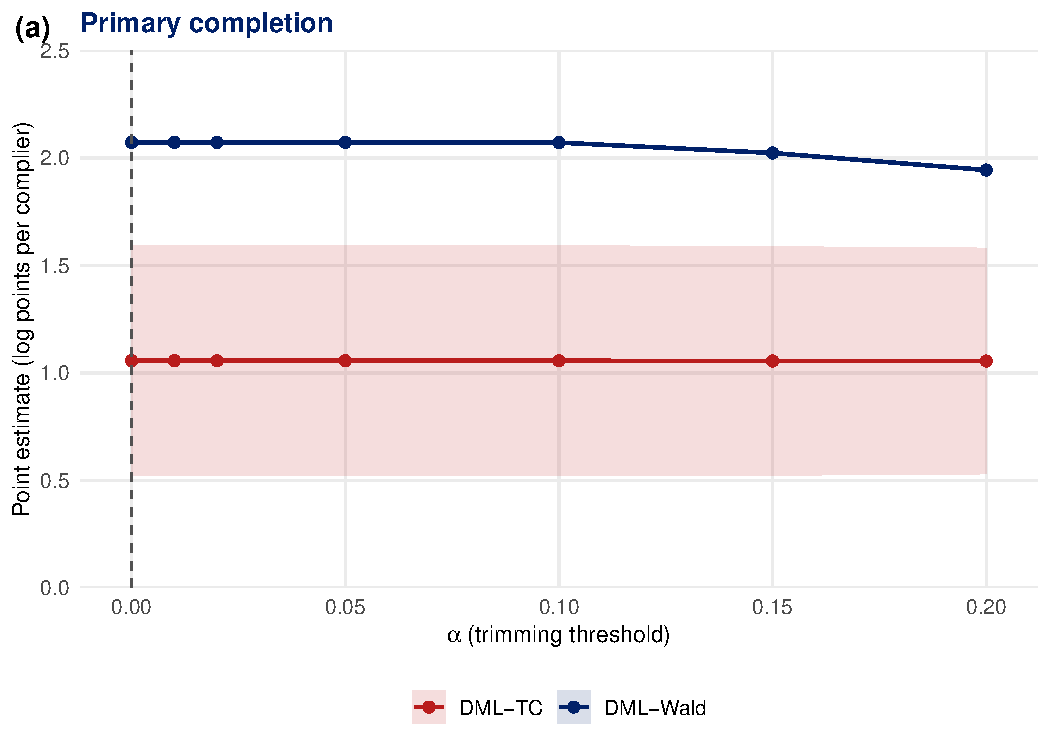
\includegraphics[width=\linewidth]{../output/figures/empirical_sensitivity_primary.pdf}
        \caption{Primary completion ($D \ge 6$).}\label{fig:sensitivity_primary}
    \end{subfigure}
    \hfill
    \begin{subfigure}[b]{0.48\linewidth}
        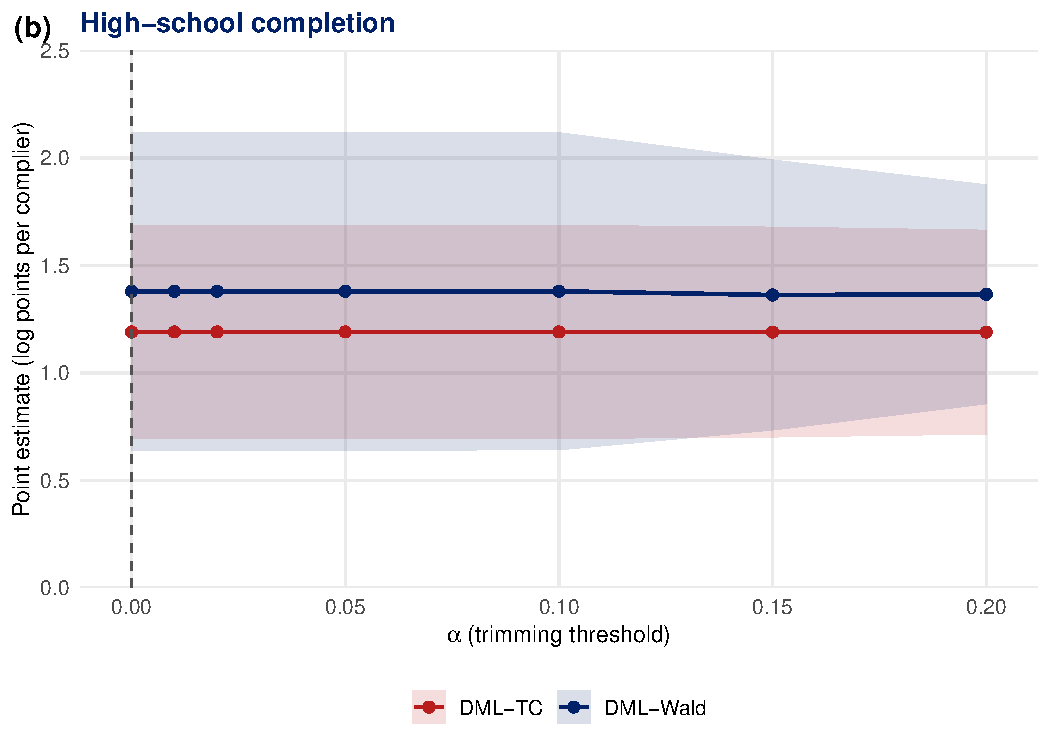
\includegraphics[width=\linewidth]{../output/figures/empirical_sensitivity_highschool.pdf}
        \caption{High-school completion ($D \ge 12$).}\label{fig:sensitivity_highschool}
    \end{subfigure}
    \caption[Sensitivity to one-sided trimming threshold]{DML-Wald and DML-TC point estimates as a function of the one-sided trimming threshold $\alpha \in [0, 0.20]$. DML-TC is flat over the full range at both margins; DML-Wald drifts but its standard error bands remain wide.}\label{fig:sensitivity_app}
\end{figure}

\begin{table}[H]
    \centering
    \small
    \input{../output/tables/empirical_4learner.tex}
    \caption[DML estimates across four first-step learners]{DML-Wald and DML-TC point estimates (cluster-robust SE in parentheses) at both treatment margins across four first-step learners. All columns use the $\hat\alpha$-rule, which returns $\hat\alpha = 0$ on the $p=45$ dictionary. DML-TC estimates agree within $0.4$ log points across learners at the primary margin and within $0.3$ at the high-school margin. DML-Wald shows more dispersion at the primary margin, reflecting the fragility of the Wald ratio under a modest first stage ($\mathrm{DID}_D = 0.088$).}\label{tab:empirical_4learner}
\end{table}
